%**************************************************************
% Valutazione Telemanom
%**************************************************************

Gli iperparametri ottimali applicati al dataset interessato hanno generato una buona soluzione come evidenziato nella
    \hyperref[tab:telemanom-metrics]{Tabella 4.3.}

    \begin{table}[H]
        \centering
        \caption{Risultati Telemanom.}
        \begin{tabular}{lr}
        \toprule
        \textbf{Soluzione Telemanom sul test set}  \\
        \midrule
        \multirow{3}{*}{\textbf{Metriche}} 
            & Precisione: 1.0 \\
            & Recall: 0.5 \\
            & F1-score: 0.66 \\
        \bottomrule
        \end{tabular}
        \label{tab:telemanom-metrics}
    \end{table}

La soluzione sembra ottima, notevolmente migliore rispetto a quelle dei modelli precedenti, tuttavia non è totalmente 
valida nella nostra applicazione e il motivo è semplice: Telemanom gestisce le anomalie, e calcola metriche su esse,
basandosi solo sugli intervalli anomali come già citato nella \hyperref[sez-telemanom]{Sottosezione 3.3.1}. Gli intervalli anomali ground-truth
nell'esperimento appena riportato sono solo due: uno grande che dura considerevolmente nel tempo, mentre l'altro 
molto più piccolo, come si evince nella \hyperref[fig:telemanom-ys-comparison]{Figura 4.1.}, in cui 
sono illustrati i valori reali e i valori previsti dal modello del dataset che rappresenta la latenza media 
delle richieste di login a Infostud. Telemanom identifica sempre e solo l'intervallo più grande come anomalo 
nei modelli dei vari canali, mentre quello più piccolo non è mai rilevato. Ciò ha portato a una soluzione che
sembra ottima, ma che in realtà, per struttura stessa del modello e dei dati che osserva, sta overfittando il 
dataset. Nella \hyperref[fig:telemanom-e_s]{Figura 4.2.} viene illustrato il grafico degli errori
smussati $\mathbf{e}_s$ riferente allo stesso segnale precedente.

\begin{figure}[H]
    \centering
    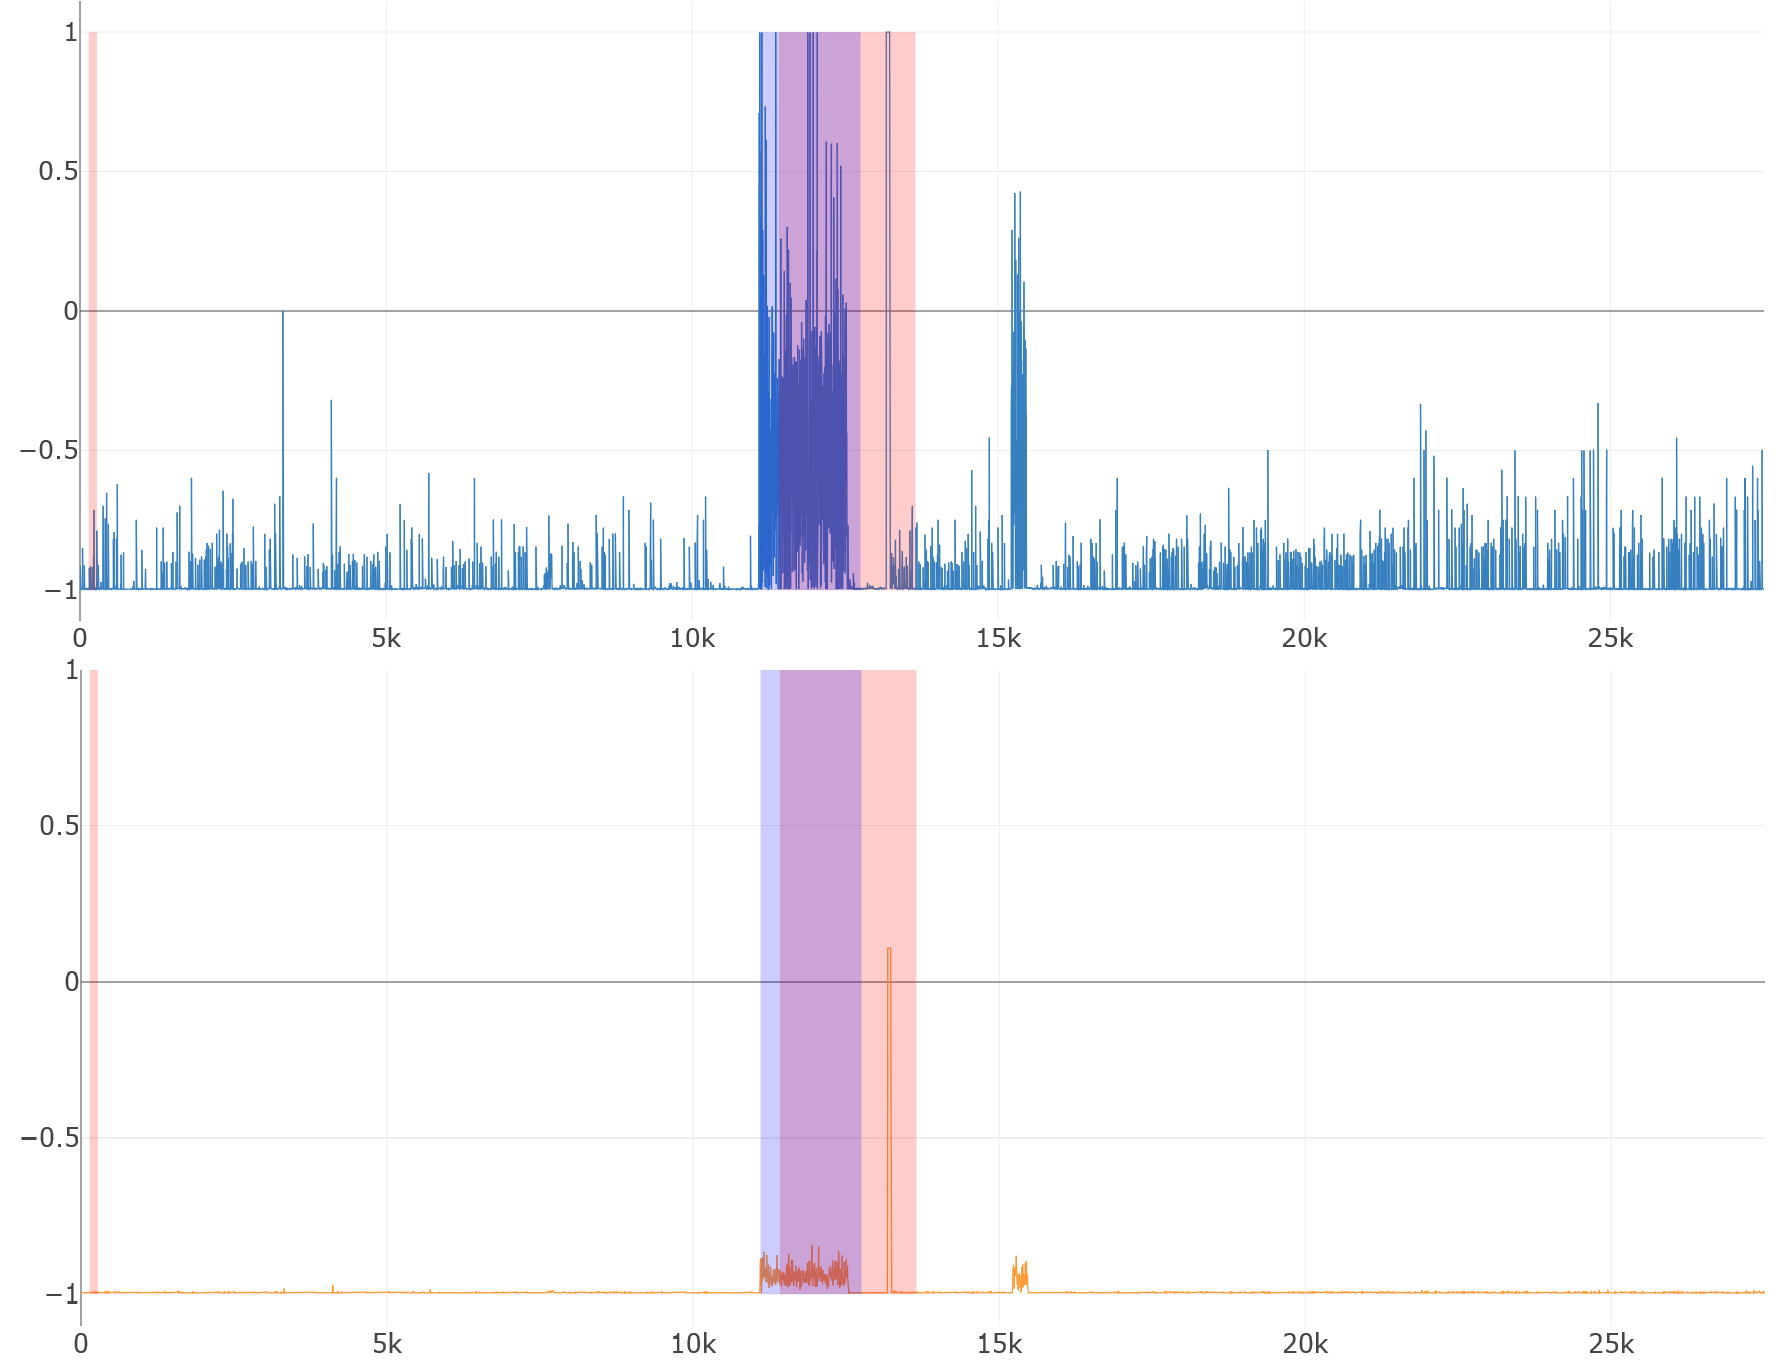
\includegraphics[width=0.7\textwidth]{./input/chapters/models/figs/telemanom-ys-comparison.png}
    \caption{Dati reali $y$ (sopra) e previsione di Telemanom $\hat{y}$ (sotto) della latenza media delle richieste
    login a InfoSapienza. Le bande rosse rappresentano periodi anomali ground-truth, la banda blu è l'intervallo 
    che il modello giudica anomalo.}
    \label{fig:telemanom-ys-comparison}
\end{figure}

\begin{figure}[H]
    \centering
    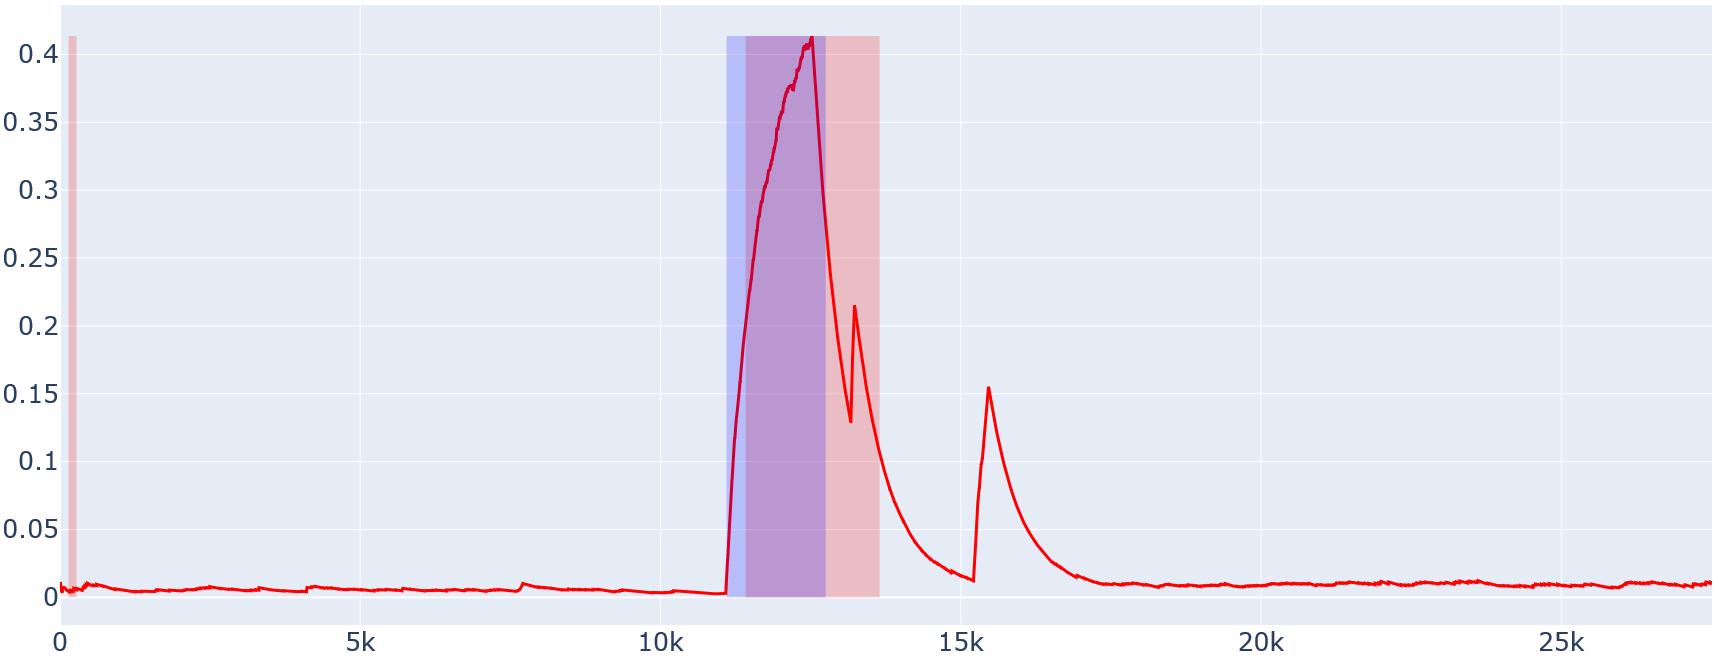
\includegraphics[width=0.7\textwidth]{./input/chapters/models/figs/telemanom-e_s.png}
    \caption{Errore smussato tra i valori reali e la previsione del modello $\mathbf{e}_s$ dei dati che rappresentano la 
    latenza media delle richieste login a InfoSapienza.}
    \label{fig:telemanom-e_s}
\end{figure}


Durante il mio studio di Telemanom ho compreso che il modello, in un contesto in cui sono presenti più anomalie 
che non durano molto nel tempo non performa in maniera altrettanto ottimale. Per riuscire a ottenere un 
discreto punteggio di recall, viene generato un grande numero di falsi positivi; i risultati rimangono coerenti 
a ciò che gli autori originali hanno descritto nel paper: Telemanom, purtroppo, genera molti falsi positivi, e non sembra che 
le sue capacità di pruning, nell'ambito di InfoSapienza, riescano a mitigare molto il problema.
    
In sintesi Telemanom, purtroppo, non si presta bene nel contesto della rilevazione di anomalie 
del dataset di Infostud. Il risultato, seppur ottimo, non viene ritenuto valido perché genera una soluzione che, 
in una situazione più naturale, sarebbe stata molto diversa.